\chapter{Algorithms: Search}

\section{Linear Search Algorithm \cite{gfg-linear-search}}\label{Linear Search Algorithm}

\begin{table}[h]
    \begin{minipage}[t]{0.5\linewidth}
        \begin{figure}[H]
            \centering
            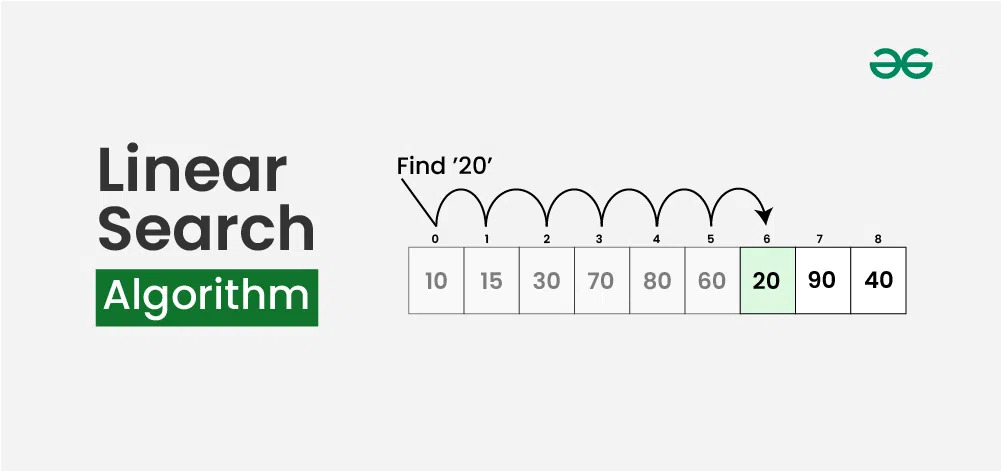
\includegraphics[width=\linewidth,height=6cm,keepaspectratio]{Pictures/ds-algo/Linear-Search-algorithm.jpg}
            \caption{Linear Search Algorithm}
        \end{figure}
    \end{minipage}
    \hfill
    \begin{minipage}[t]{0.35\linewidth}
        \begin{table}[H]
            \begin{tabular}{l l l}
                \multicolumn{3}{c}{\textbf{Time Complexity}} \\
                 Best Case & $O(1)$ & first index \\
                 Average Case & $O(N)$ &  \\
                 Worst Case & $O(N)$ & last index \\
                 \multicolumn{3}{c}{\textbf{Space Complexity}}\\
                 Auxiliary Space & $O(1)$ & iterator \\
            \end{tabular}
        \end{table}
    \end{minipage}
\end{table}

\textbf{Steps}:
\begin{enumerate}
    \item \textbf{Start}: Begin at the first element of the collection of elements.
    \item \textbf{Compare}: Compare the current element with the desired element.
    \item \textbf{Found}: If the current element is equal to the desired element, return true or index to the current element.
    \item \textbf{Move}: Otherwise, move to the next element in the collection.
    \item \textbf{Repeat}: Repeat steps 2-4 until we have reached the end of collection.
    \item \textbf{Not found}: If the end of the collection is reached without finding the desired element, return that the desired element is not in the array.
\end{enumerate}

\begin{table}[h]
    \begin{minipage}[t]{0.48\linewidth}
        \textbf{Advantages}:
        \begin{itemize}
            \item Linear search can be used irrespective of whether the array is sorted or not. 
            \item It can be used on arrays of any data type.
            \item Does not require any additional memory.
            \item It is a well-suited algorithm for small datasets.
        \end{itemize}
    \end{minipage}
    \hfill
    \begin{minipage}[t]{0.48\linewidth}
        \textbf{Disadvantages}:
        \begin{itemize}
            \item Linear search has a time complexity of $O(N)$, which in turn makes it \textbf{SLOW} for large datasets.
            \item \textbf{NOT} suitable for large arrays.
        \end{itemize}
    \end{minipage}
\end{table}

\begin{lstlisting}[language=Python, caption=Linear Search Algorithm - Python]
def search(arr: list, N: int, x: object) -> int:
    for i in range(0, N):
        if (arr[i] == x):
            return i
    return -1
\end{lstlisting}

\section{Binary Search Algorithm \cite{gfg-binary-search}} \label{Binary Search Algorithm}

\begin{table}[H]
    \begin{minipage}[t]{0.45\linewidth}
        \begin{figure}[H]
            \centering
            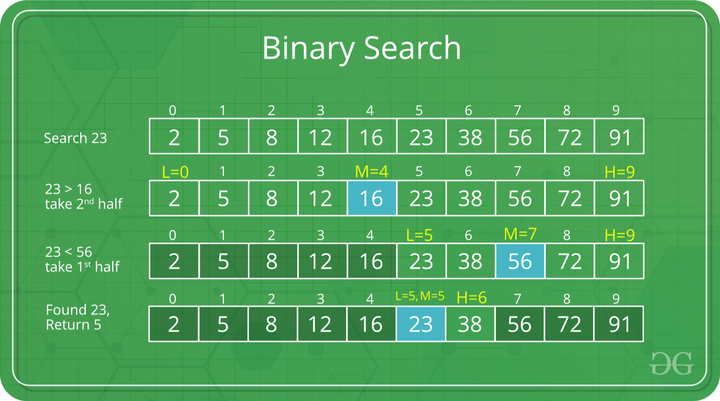
\includegraphics[width=\linewidth,height=6cm,keepaspectratio]{Pictures/ds-algo/BinarySearch.png}
            \caption{Binary Search Algorithm}
        \end{figure}
    \end{minipage}
    \hfill
    \begin{minipage}[t]{0.55\linewidth}
        \begin{table}[H]
            \begin{tabular}{l l l}
                \multicolumn{3}{c}{\textbf{Time Complexity}} \\
                 Best Case & $O(1)$ & \\
                 Average Case & $O(\log(N))$ &  \\
                 Worst Case & $O(\log(N))$ &  \\
                 \multicolumn{3}{c}{\textbf{Space Complexity}}\\
                 Auxiliary Space & $O(1)$ & \\
                 Auxiliary Space & $O(\log(N))$ & recursive call stack \\
            \end{tabular}
        \end{table}
    \end{minipage}
\end{table}


\textbf{Steps}:
\begin{enumerate}
    \item Divide the search space into two halves by finding the middle index “mid”.
    \item Compare the middle element of the search space with the key.
    \item If the key is found at middle element, the process is terminated.
    \item If the key is not found at middle element, choose which half will be used as the next search space.
    \begin{enumerate}
        \item If the key is smaller than the middle element, then the left side is used for next search.
        \item If the key is larger than the middle element, then the right side is used for next search.
    \end{enumerate}
    \item This process is continued until the key is found or the total search space is exhausted.
\end{enumerate}

\begin{table}[h]
    \begin{minipage}[t]{0.48\linewidth}
        \textbf{Advantages}:
        \begin{itemize}
            \item Binary search is faster than linear search, especially for large arrays.
            \item More efficient than other searching algorithms with a similar time complexity, such as interpolation search or exponential search.
            \item Binary search is well-suited for searching large datasets that are stored in external memory, such as on a hard drive or in the cloud.
        \end{itemize}
    \end{minipage}
    \hfill
    \begin{minipage}[t]{0.48\linewidth}
        \textbf{Disadvantages}:
        \begin{itemize}
            \item The array should be \textbf{sorted}.
            \item Binary search requires that the data structure being searched be stored in contiguous memory locations. 
            \item Binary search requires that the elements of the array be comparable, meaning that they must be able to be ordered.
        \end{itemize}
    \end{minipage}
\end{table}

\begin{lstlisting}[language=Python, caption=Binary Search (iterative) - Python]
def binarySearch(arr: list, low: int, high: int, x: object) -> int:
    while low <= high:
        mid = low + (high - low) // 2

        # Check if x is present at mid
        if arr[mid] == x: return mid

        # If x is greater, ignore left half
        elif arr[mid] < x: low = mid + 1

        # If x is smaller, ignore right half
        else: high = mid - 1

    # If we reach here, then the element was not present
    return -1
\end{lstlisting}

\begin{lstlisting}[language=Python, caption=Binary Search (recursive) - Python]
def binarySearch(arr: list, low: int, high: int, x: object) -> int:
    # Check base case
    if high >= low:
        mid = low + (high - low) // 2
        
        # If element is present at the middle itself
        if arr[mid] == x: return mid
            
        # If element is smaller than mid, then it
        # can only be present in left subarray
        elif arr[mid] > x: 
            return binarySearch(arr, low, mid-1, x)

        # Else the element can only be 
        # present in right subarray
        else: return binarySearch(arr, mid + 1, high, x)

    # Element is not present in the array
    else: return -1
\end{lstlisting}

\section{Ternary Search \cite{gfg-ternary-search}}\label{Ternary Search}
\begin{table}[h]
    \begin{minipage}{0.5\linewidth}
        \begin{figure}[H]
            \centering
            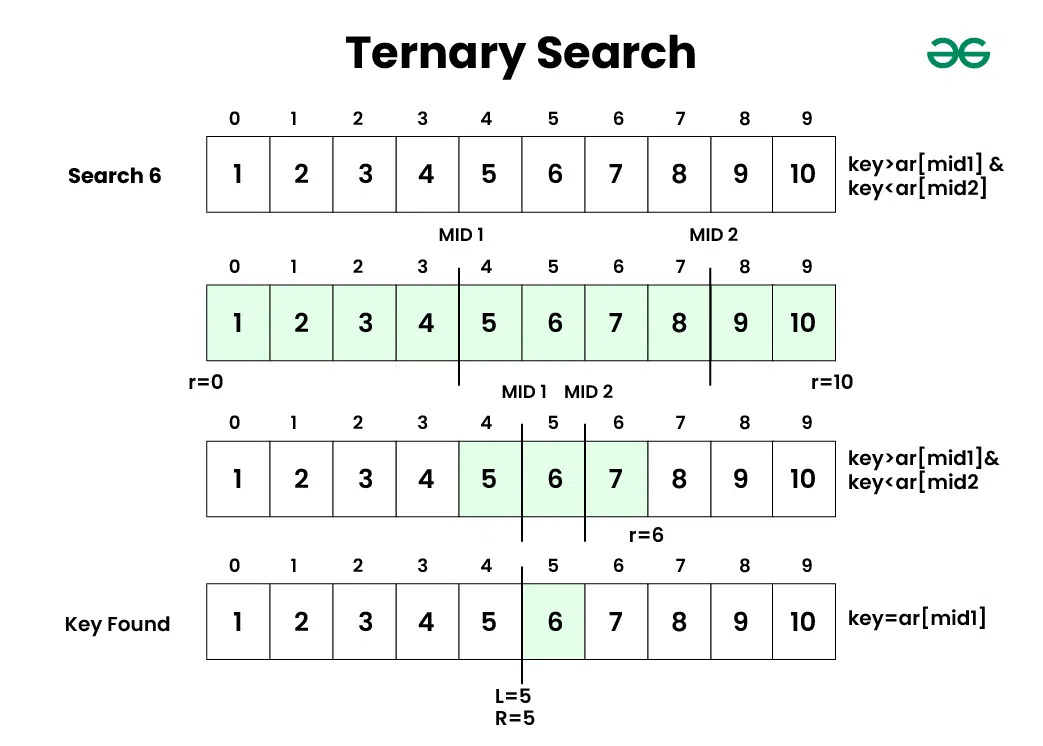
\includegraphics[width=\linewidth, height=10cm, keepaspectratio]{Pictures/ds-algo/Ternary-Search.jpg}
            \caption{Ternary Search}
        \end{figure}
    \end{minipage}
    \hfill
    \begin{minipage}{0.47\linewidth}
        \begin{table}[H]
            \begin{tabular}{l l l}
                \multicolumn{3}{c}{\textbf{Time Complexity}} \\
                 Recursive & $O(2*\log_3(N))$ & \\
                 Iterative & $O(\log_3(N))$ & \\
                 \multicolumn{3}{c}{\textbf{Space Complexity}}\\
                 Auxiliary Space & $O(2*\log_3(N))$ & Recursive \\
                 Auxiliary Space & $O(1)$ & Iterative \\
            \end{tabular}
        \end{table}
    \end{minipage}
\end{table}

\vspace{0.2cm}
\textbf{Steps}:
\begin{enumerate}
    \item \textbf{Initialization}: Set two pointers, \textbf{left} and \textbf{right}, initially pointing to the first and last elements of our search space.

    \item \textbf{Divide the search space}:
    \begin{enumerate}
        \item Calculate two midpoints, mid1 and mid2, dividing the current search space into three roughly equal parts:
        \item[] $mid1 = left + (right - left) / 3$
        \item[] $mid2 = right - (right - left) / 3$
        \item The array is now effectively divided into $[left, mid1]$, $(mid1, mid2)$, and $[mid2, right]$.
    \end{enumerate}

    \item \textbf{Comparison with Target}:
    \begin{enumerate}
        \item If the \textbf{target} is equal to the element at \textbf{mid1} or \textbf{mid2}, the search is successful, and the index is returned.

        \item If the target is less than the element at mid1, update the right pointer to $mid1 - 1$.

        \item If the target is greater than the element at mid2, update the left pointer to $mid2 + 1$.

        \item If the target is between the elements at mid1 and mid2, update the left pointer to $mid1 + 1$ and the right pointer to $mid2 - 1$.
    \end{enumerate}

    \item \textbf{Repeat or Conclude}:
    \begin{enumerate}
        \item Repeat the process with the reduced search space until the target is found or the search space becomes empty.

        \item If the search space is empty and the target is not found, return a value indicating that the target is not present in the array.
    \end{enumerate}
\end{enumerate}

\begin{table}[h]
    \begin{minipage}[t]{0.48\linewidth}
        \textbf{Advantages}:
        \begin{itemize}
            \item Ternary search can find maxima/minima for unimodal functions, where binary search is not applicable.
            
            \item Ternary Search has a time complexity of $O(2 * \log_3(N))$, which is more efficient than linear search and comparable to binary search.

            \item Fits well with optimization problems.
        \end{itemize}
    \end{minipage}
    \hfill
    \begin{minipage}[t]{0.48\linewidth}
        \textbf{Disadvantages}:
        \begin{itemize}
            \item Ternary Search is only applicable to ordered lists or arrays, and cannot be used on unordered or non-linear data sets.

            \item Ternary Search takes more time to find maxima/ minima of monotonic functions as compared to Binary Search.
        \end{itemize}
    \end{minipage}
\end{table}

\begin{lstlisting}[language=Python, caption=Ternary Search (recursive) - Python]
def ternarySearch(l: int, r: int, key: int, ar: list) -> int:
    if (r >= l):
        # Find the mid1 and mid2
        mid1 = l + (r - l) //3
        mid2 = r - (r - l) //3

        # Check if key is present at any mid
        if (ar[mid1] == key):  return mid1
        
        if (ar[mid2] == key): return mid2
        
        # Since key is not present at mid,
        # check in which region it is present
        # then repeat the Search operation
        # in that region
        if (key < ar[mid1]): 
            # The key lies in between l and mid1
            return ternarySearch(l, mid1 - 1, key, ar)
        
        elif (key > ar[mid2]): 
            # The key lies in between mid2 and r
            return ternarySearch(mid2 + 1, r, key, ar)
        
        else: 
            # The key lies in between mid1 and mid2
            return ternarySearch(mid1 + 1, mid2 - 1, key, ar)
        
    # Key not found
    return -1
\end{lstlisting}
\begin{lstlisting}[language=Python, caption=Ternary Search (iterative) - Python]
def ternarySearch(l: int, r: int, key: int, ar: list) -> int:
    while r >= l:
        # Find mid1 and mid2
        mid1 = l + (r-l) // 3
        mid2 = r - (r-l) // 3

        # Check if key is at any mid
        if key == ar[mid1]: return mid1
        if key == ar[mid2]: return mid2

        # Since key is not present at mid, 
        # Check in which region it is present
        # Then repeat the search operation in that region
        if key < ar[mid1]:
            # key lies between l and mid1
            r = mid1 - 1
        elif key > ar[mid2]:
            # key lies between mid2 and r
            l = mid2 + 1
        else:
            # key lies between mid1 and mid2
            l = mid1 + 1
            r = mid2 - 1

    # key not found
    return -1
\end{lstlisting}


\section{Exponential Search \cite{gfg-exponential-search}}\label{Exponential Search}

\begin{table}[h]
    \begin{tabular}{l l l}
         \textbf{Time Complexity} & $O(\log(N))$ &  \\
         \multicolumn{3}{c}{\textbf{Space Complexity}}\\
         Auxiliary Space & $O(1)$ & iterative \\
         Auxiliary Space & $O(\log(N))$ & recursive \\
    \end{tabular}
\end{table}

\textbf{Steps}:
\begin{enumerate}
    \item Find range where element is present
    \item Do \fullref{Binary Search Algorithm} in above found range
\end{enumerate}

\begin{lstlisting}[language=Python, caption=Exponential Search - Python]
# Returns the position of first occurrence of x in array
def exponentialSearch(arr: list, n: int, x: object) -> int:
    # IF x is present at first 
    # location itself
    if arr[0] == x: return 0
         
    # Find range for binary search 
    # j by repeated doubling
    i = 1
    while i < n and arr[i] <= x: i = i * 2
     
    # Call binary search for the found range
    return binarySearch(arr, i // 2, min(i, n-1), x)
\end{lstlisting}


\section{Selective Search (CNN) \cite{https://www.geeksforgeeks.org/r-cnn-region-based-cnns/}}\label{Selective Search (CNN)}

\begin{table}[h]
    \begin{minipage}[t]{0.39\linewidth}
        \begin{figure}[H]
            \centering
            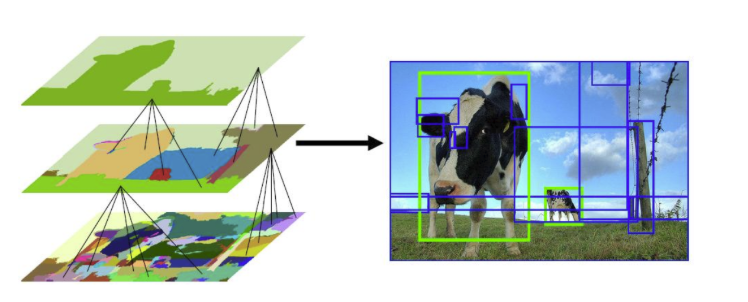
\includegraphics[width=\linewidth, height=3cm, keepaspectratio]{Pictures/convolutional-neural-network/rcnn-selective-search.png}
            \caption{Selective Search}
        \end{figure}        
    \end{minipage}
    \hfill
    \begin{minipage}[t]{0.59\linewidth}
        \begin{itemize}
            \item Selective search is a \textbf{greedy algorithm} that combines smaller segmented regions to generate region proposals.
            
            \item This algorithm takes an image as input and output generates region proposals on it.
        
            \item This algorithm has the advantage over random proposal generation in that it limits the number of proposals to approximately 2000 and these region proposals have a high recall.
        \end{itemize}    
    \end{minipage}
\end{table}


\vspace{0.2cm}
\textbf{Algorithm}:
\begin{enumerate}
    \item Generate initial sub-segmentation of the input image.

    \item Combine similar bounding boxes into larger ones recursively.

    \item Use these larger boxes to generate region proposals for object detection.
\end{enumerate}

\vspace{0.2cm}
\textbf{Challenges}:
\begin{enumerate}
    \item The selective Search algorithm is very rigid and there is no learning happening in that. This sometimes leads to bad region proposal generation for object detection.
\end{enumerate}
































